\subsection{Teil 1 - Klassifizierung von Rechnungen}

In diesem Kapitel werden zwei Experimente erläutert, mit welchen die Klassifizierung von Rechnungen ermöglicht werden soll. Das erste Experiment ist ein Bild-basierter und das zweite ein Text-basierter Ansatz zur Klassifizierung von Rechnungen. Die Klassifizierung dient dazu, eine Rechnung einer bestimmten Art (Klasse) zuzuweisen. Die Klassen Optiker und Fitness sind durch die Anforderungen gegeben. Neben diesen Klassen könnten Rechnungen noch in viele weitere Klassen eingeteilt werden. Um die Erweiterbarkeit des Modells um weitere Klassen zu prüfen, wird eine zusätzliche Klasse eingeführt. In diesem Experiment werden Rechnungen in die Klassen Optiker, Fitness, Sportverein und Andere eingeteilt. Zu einem späteren Zeitpunkt wäre es denkbar, die Anzahl Klassen zu erhöhen und somit auch andere Arten von Rechnungen zu automatisieren.

Der Ausgangspunkt für die Klassifizierung ist ein Bild einer Rechnung. Die Klassifizierung von Bildern respektive Fotos ist eine bekannte Problematik der Computer Vision und bildet in diesem Bereich die Grundlage für die Lösung vieler weiterer Problematiken~\autocite{StanfordGithubClassification}. 

% Die Wichtigkeit der Bildklassifizierung zeigt die Organisation ImageNet. ImageNet aht es zum Ziel, Forschern einen einfachen Zugang zu Datensätzen von Bildern zu gewähren. Seit 2010 wurden bereits sieben Wettbewerbe im Bereich der Computer Vision veranstaltet rund um die Klassifizierung von Bildern und die Erkennung von Objekten auf diesen Bildern~\autocite{ImageNet2019}. 

Es liegt nahe, die Klassifizierung der Rechnungen mit Bild-basierten Modellen aus dem Bereich der Computer Vision anzugehen. Dieser Ansatz wird im folgenden Kapitel erläutert.

Nicht nur im Bereich der Computer Vision ist die Problematik der Klassifizierung ein viel behandeltes Themengebiet. Im Bereich des Natural Language Processing ist die Klassifizierung von Wörtern, Sätzen oder ganzen Texten eine bekannte Problemstellung. Die sogenannte Text Classification ist die Grundlage für viele Applikationen, welche mit Texten arbeiten. So verwenden beispielsweise Mail-Server Text Classification, um zu entscheiden, ob ein E-Mail Spam ist oder nicht~\autocite{GoogleTextClassification}

Im Kapitel \ref{chap:text-based-classification} wird die Text-basierte Klassifizierung der Rechnungen weiterverfolgt.

Die beiden Ansätze zur Klassifizierung werden anhand der knapp 24'500 bereits bei der AXA eingereichten Rechnungen evaluiert. Um dies zu ermöglichen, wurden die Rechnungen aus dem System der AXA exportiert und in die oben genannten Klassen eingeteilt. 

Der Datensatz musste auf 17'196 Rechnungen reduziert werden. Etwas mehr als 7'000 Rechnungen hatten mehr als eine Seite. Aus diesem Grund konnten diese Rechnungen mit den vorhandenen Informationen nicht eindeutig einer Klasse zugewiesen werden. Eine manuelle Klassifizierung würde für den Umfang dieses Experiments einen zu grossen Arbeitsaufwand darstellen.

Bei der Durchsicht der Rechnungen wurden 127 Rechnungen aufgrund mangelnder Qualität aussortiert. Diese Problematik wird durch die vor kurzem eingeführte Qualitätsprüfung (vgl. Abbildung \ref{prozessaxa}) nicht mehr vorkommen und ist deshalb für diese Arbeit nicht weiter relevant.

Nach der Einteilung in die vier Klassen ist festzustellen, dass die 17'196 Rechnungen eine sehr unregelmässige Verteilung aufweisen (vgl. Abbildung. \ref{class-distribution}). Die Klasse Sportverein ist gegenüber den anderen Klassen mit nur 760 Rechnungen unterrepräsentiert. Die Klasse Andere ist hingegen mit 12751 Rechnungen überrepräsentiert. Es ist wichtig, diesem Umstand während dem Training eines Modells Rechnung zu tragen. Ansonsten würde die Voraussage des Modells zu oft in der überrepräsentierten Klasse Andere resultieren. Diese Problematik kann auf diverse Arten angegangen werden. In dieser Arbeit wird dazu eine, aufgrund der Klassenverteilung, gewichtete Loss Funktion verwendet~\autocite{Buda2018}.

\begin{figure}[h]
    \captionsetup{width=.9\linewidth}
    \caption{Ungleichverteilung der Klassen innerhalb des Trainingsdatensatzes}
    \label{class-distribution}
    \centering
    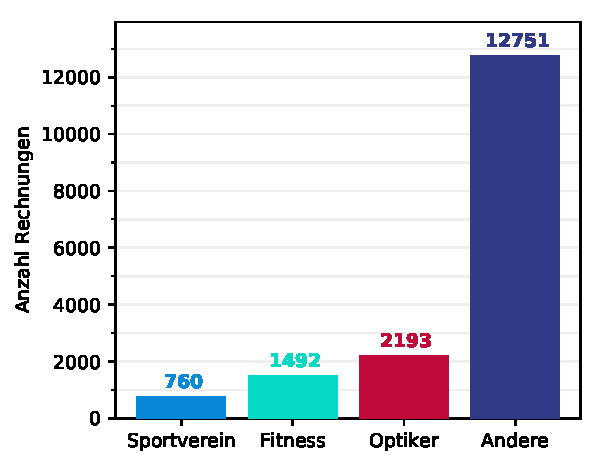
\includegraphics[scale=1]{graphics/matplot/class-weight.pdf}
\end{figure}
